\documentclass[10pt]{article}
\usepackage[utf8]{inputenc}
\usepackage{url}
\usepackage{hyperref}
\usepackage{amsmath}
\usepackage{amsfonts}
\usepackage{amssymb}
\usepackage{graphicx}
\graphicspath{ {./images/} }
\usepackage{float}
\usepackage{lipsum}
\usepackage{sectsty}
\usepackage{tikz}
\sectionfont{\centering}
\usepackage{multicol}
\usepackage{xcolor}
\usepackage{natbib}
\usepackage{graphicx}
\usepackage{listings}
\usepackage{xcolor}
\usepackage{pgfplots}
\usepackage[font=small]{caption}
\addtolength{\abovecaptionskip}{-3mm}
\addtolength{\textfloatsep}{-5mm}
\setlength\columnsep{20pt}

\usepackage[a4paper,left=1.50cm, right=1.50cm, top=2cm, bottom=3cm]{geometry}


\author{}

\title{\Large{Design and Analysis of Algorithms Assignment - 6}}
\begin{document}
	\begin{center}
		{\Large \textbf{Design and Analysis of Algorithms Assignment - 6}}\\
		\vspace{1em}
		{\large Department of Information Technology}\\
		\vspace{1em}
		\large{Indian Institute of Information Technology - Allahabad, India}\\
		\vspace{1em}
		\large{Gitika Yadav \hspace{10em} Divyatez Singh \hspace{10em} Divyansh  Rai}
		\large{IIT2019219 \hspace{10.5em} IIT2019220 \hspace{10.5em} IIT2019221}
		
		\vspace{2.5em}
	\end{center}
	
\begin{multicols*}{2}

    \textbf{\emph{{Abstract}:This paper introduces an algorithm that calculates the minimum  distance between any pair location(or cells) in a given 2D matrix(with all 0’s and 1’s, 0 denoting blocked cells) .
}}\\
	
	\textbf{\emph{{Index Terms}: 2D-Arrays, Queue, Recursion\\}}


\section*{INTRODUCTION}
 

Breadth-first search (BFS) is an algorithm for traversing or searching graphs or trees , by exploring all of the neighbor nodes at the present depth prior to moving on to the nodes at the next depth level.



\paragraph{Breadth First Search}

Breadth first search is a general technique of traversing a graph. Breadth first search may use more memory but will always find the shortest path first. It is a path finding algorithm that is capable of always finding the solution if one exists.


\begin{enumerate}
    \item\textbf{Data Structure:}  In this search a queue data structure is used and it is level by level traversal.
    \item\textbf{Traversal:}  Breadth first search expands nodes in order of their distance from the root.
    \item\textbf{Path:} Each node in the search tree is expanded in a breadth wise at each level.\\\\
\end{enumerate}

\includegraphics[width=\columnwidth, height=8cm]{bfs.png}\begin{center}\textbf{Figure 1:} Divide and Conquer\end{center}


\paragraph{Advantages of Breadth-first search}
The Breadth-first search technique generally has following mentioned advantages over Brute Force Algorithms.\\\\
\textbf{Time Efficiency} Used to find the shortest path between vertices as traverses by level in shortest time.\\\\
\textbf{Space Efficiency:} As no need to mention the algorithm,  but still, the space complexity also reduces up to a much extent due to the nature of searching level by level\\

\\This report further contains:
\begin{itemize}
\item 	Algorithm  Designs
\item 	Algorithm  Analysis
\item 	Experimental Study and Profiling
\item 	Conclusion
\item 	References
\item 	Appendix
\end{itemize}

\section*{ALGORITHM DESIGN}
A general problem based on the breath-first search in which, we level order traversal nodes , initiating by pushing into queue and then make decisions while traveling front of queue.Following structures have been taken into account while making the code for the report.

\paragraph{Algorithmic Steps:}

For the given problem, we are given the dimension of the given matrix, then the matrix and then then for a given pair location(of cells), we need to find the shortest path from source point to destination point. 

The approach we discussed is based on Breadth First Search Algorithm for finding shortest path between two given cells, generally has the steps defined in following algorithmic procedure, which have been implemented while solving the problem:
\begin{enumerate}

\item	Input dimension of given matrix. 
\item	Store then the matrix and source cell’s and destination cell’s location.
\item	Store each cell as a node with their row, column values and distance from the source cell.
\item	Start BFS with the source cell.

\item Make a visited array with all having “false” values.
\item Keep updating distance from source value in each move.
\item Return distance when destination is met, else return -1 (no path exists in between source and destination).
\end{enumerate}

The above returned cost is the sum of distance from source to destination.

\lstset { %
    language=C++,
    backgroundcolor=\color{black!5},
    basicstyle=\footnotesize,
}

\begin{lstlisting}
        
Int:
procedure main 
	n ->row
	m ->column
	a[n][m]->matrix with input
	si,sj ->source cell location
    di,dj ->destination cell location

    if(source cell or destination cell equals 0):
    	print(“Path not possible”)
    
    else:
    	Initialize queue (of pair of int) q
    	Initialize vector vis[n][m] with all 
    	values initially false
    	
    	Initialize cost -> 0
    	set vis[si][sj] -> true
    	push ({si,sj}) in q
    
    	while(q.size()>0):
    		cost++
    		p -> q.size
    		
    		while(p--):
    			top -> q.front()
            q.pop()
            x->top.first	
    		y->top.second
    		
    		
    			
    	if(x>0):
    		if(valid left cell):
    			Left node visited
    			Queue push left node  
    	if(y>0):
    		if(valid above cell ):
    			Above node visited
    			Queue push above node
    	if(x<n-1):
    		if(valid right cell ):
    			Right node visited
    			Queue push right cell  
    	if(x>0):
    		if(valid below cell ):
    			Below node visited
    			Queue push below cell 
    		
    	if(destination cell is visited):
    		print(cost)
    		break
    	End of while
    	
    	if(destination cell is visited):
    		break
    End of while
    if(destination still not visited):
    	print(“Not Found”)

End of procedure



\end{lstlisting}
    

	\includegraphics[width=8cm, height=8cm]{12.png}\begin{center}\textbf{Figure 2:} BFS Traversal \end{center}

\section*{ALGORITHM ANALYSIS} 
	
\paragraph{APRIORI ANALYSIS :}\\
This is the analysis performed prior to running in a stage where the function is defined using a theoretical model. Therefore, complexity is determined by just examining the algorithm rather than running it on a particular system with a different memory,processor, and compiler. So,as we discussed under the heading complexity analysis we arrived at the conclusion that the best time complexity is O(1) and the space complexity O(n*m).

\paragraph{Time complexity Derivation:} Let Time complexity of above algorithm be T(n) and it can be expressed as follows:\\
\textbf{TIME COMPLEXITY DERIVATION:}
\rule{9cm}{1pt}
\textit{
T(n) = V (O(1) + O(Edge from vertex) + O(1))\\\\
As each vertex can travel in 4 directions:\\
T(n) = V + 4V  + V\\
T(n) = 2V + E(total number of edges in graph)\\
T(n) = V + E \\
\\
Scanning for all adjacent vertices takes O(E) time, since sum of lengths of adjacency lists is E.\\
Thus on combining we get the overall time 
complexity as:T(n) = O(V+E)\\}
\rule{9cm}{1pt}

\includegraphics[width=8cm, height=8cm]{13.png}\begin{center}\textbf{Figure 2:} Time Complexity Derivation  \end{center}
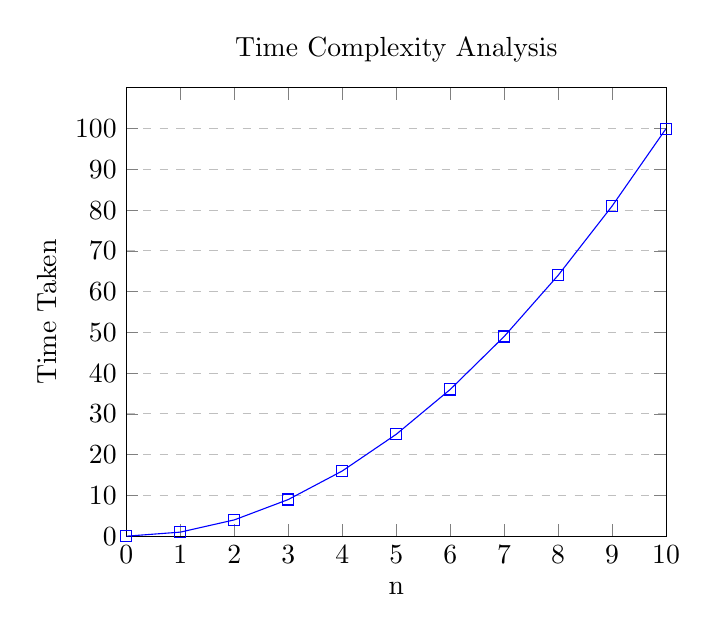
\begin{tikzpicture}
\begin{axis}[
    title={Time Complexity Analysis},
    xlabel={n},
    ylabel={Time Taken},
    xmin=0, xmax=10,
    ymin=0, ymax=110,
    xtick={0,1,2,3,4,5,6,7,8,9,10},
    ytick={0,10,20,30,40,50,60,70,80,90,100},
    legend pos=north west,
    ymajorgrids=true,
    grid style=dashed,
]

\addplot[
    color=blue,
    mark=square,
    ]
    coordinates {
    (0,0)(1,1)(2,4)(3,9)(4,16)(5,25)(6,36)(7,49)(8,64)(9,81)(10,100)
    };
    
\end{axis}
\end{tikzpicture}
\paragraph{Time Analysis:}Following is the graph representing the time complexity of the algorithm.\\\\\\

By the experimental analysis, we found that in  case of optimized approach, on increasing the number of numbers the graph is strictly increasing with a bend (or concavity) towards horizontal axis. Thus the overall time increases with an increase in size.



\paragraph{Space Analysis:}Following is the graph representing the space complexity of the algorithm.\\\\
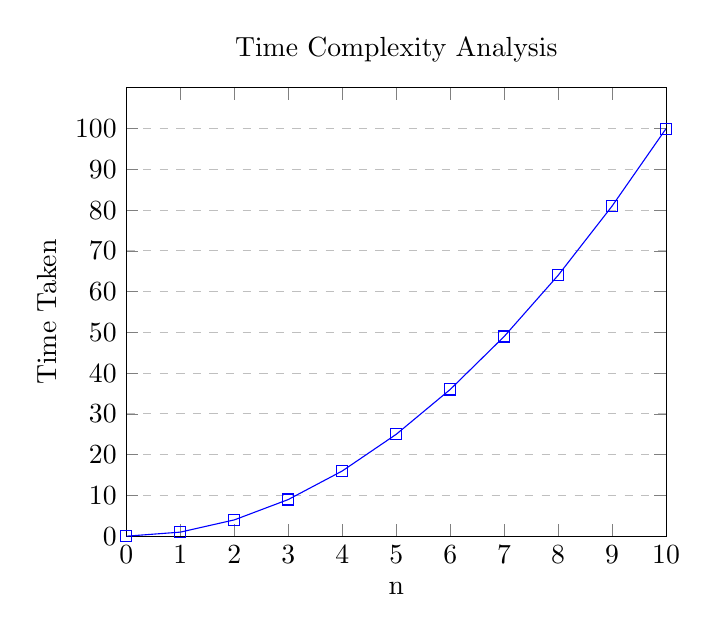
\begin{tikzpicture}
\begin{axis}[
    title={Time Complexity Analysis},
    xlabel={n},
    ylabel={Time Taken},
    xmin=0, xmax=10,
    ymin=0, ymax=110,
    xtick={0,1,2,3,4,5,6,7,8,9,10},
    ytick={0,10,20,30,40,50,60,70,80,90,100},
    legend pos=north west,
    ymajorgrids=true,
    grid style=dashed,
]

\addplot[
    color=blue,
    mark=square,
    ]
    coordinates {
    (0,0)(1,1)(2,4)(3,9)(4,16)(5,25)(6,36)(7,49)(8,64)(9,81)(10,100)
    };
    
\end{axis}
\end{tikzpicture}

By the experimental analysis, we found that in case of optimized approach, on increasing the number of numbers the graph is strictly increasing. Thus the overall space increases with an increase in size.\\

\includegraphics[width=8cm, height=8cm]{11.png}\begin{center}\textbf{Figure 2:} Worst Case Time Complexity \end{center}

\includegraphics[width=8cm, height=8cm]{14.png}\begin{center}\textbf{Figure 2:} Best Case Time Complexity \end{center}


\paragraph{APOSTERIORI ANALISIS:}
Aposteriori analysis of an algorithm means we per- form analysis of an algorithm only after running it on a system. It directly depends on the system and changes from system to system. So for the a aposteriori analysis of the algorithm,we have run our code on the compiler and get values of the time.
% \includegraphics[width=\columnwidth, height=6cm]{time_2.jpeg}\begin{center}\textbf{Figure 5:} Time Complexity Graph\end{center}
\section*{Experimental Analysis}
In the following table some cases are plotted for the algorithm on our local machine,
\begin{center}
 \begin{tabular}{||c | c||} 
 \hline
 n,m & Time Taken (in ms) \\ [0.5ex] 
 \hline\hline
 
 100 & 0.0039 \\
 \hline
 1000 & 0.037 \\
 \hline
 5000 & 0.058 \\ [1ex] 
 \hline
 
\end{tabular}
\end{center}

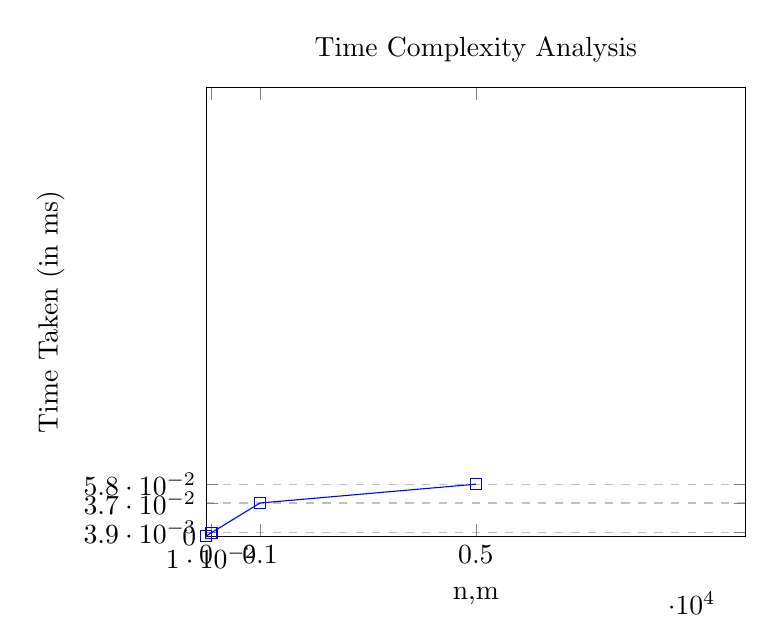
\begin{tikzpicture}
\begin{axis}[
    title={Time Complexity Analysis},
    xlabel={n,m},
    ylabel={Time Taken (in ms)},
    xmin=0, xmax=10000,
    ymin=0, ymax=0.5,
    xtick={0,100,1000,5000},
    ytick={0,0.0039, 0.037,0.058},
    legend pos=north west,
    ymajorgrids=true,
    grid style=dashed,
]

\addplot[
    color=blue,
    mark=square,
    ]
    coordinates {
    (0,0)(100,0.0039)(1000,0.037)(5000,0.058)
    };
    
\end{axis}
\end{tikzpicture}

\section*{CONCLUSION}

So, with the above mentioned algorithms and their profiling, we come to the conclusion that this minimum  distance between any pair location(or cells) in a given 2D matrix(with all 0’s and 1’s, 0 denoting blocked cells)  is achieving its best time complexity of O(V+E) and space complexity of O(V*V).\\Also, when we are dealing with large numbers such as the one occupying 64-bits (long long integers), the complexity is same. So we can take the modulus of distance with 109+7 in order to make sure that it gets fit in the available data types(long long integer types more specifically).


\section*{REFERENCES}

\begin{enumerate}
\item Introduction to Algorithms by Cormen,Charles, Rivest and Stein:\\
https://web.ist.utl.pt/~fabio.ferreira/material/asa
\item Breadth First Search or BFS for a Graph:\\
https://www.geeksforgeeks.org/breadth-first-search-or-bfs-for-a-graph/
\item Intro to BFS:\\
https://cp-algorithms.com/graph/breadth-first-search.html
\end{enumerate}\\

\section*{APPENDIX}
\textbf{To run the code, follow the following procedure:}
\begin{enumerate}
    \item Download the code(or project zip file) from the github repository.
    \item Extract the zip file downloaded above.
    \item Open the code with any IDE like Sublime Text, VS Code, Atom or some online compilers like GDB.
    \item Run the code following the proper running commands(vary from IDE to IDE)
    \begin{enumerate}
        \item \textbf{For VS Code:} Press Function+F6 key and provide the input on the terminal.
        \item \textbf{For Sublime Text:} Click on the Run button and provide the input.\\
    \end{enumerate}
\end{enumerate}
\textbf{Code for Implementation is:}
\lstset { %
    language=C++,
    backgroundcolor=\color{black!5},
    basicstyle=\footnotesize,
}

\begin{lstlisting}
#include<bits/stdc++.h>
using namespace std;


int main(){
  int n ,m;cin>>n>>m;
  int a[n][m];
   for(int i=0;i<n;i++){
	for(int j=0j<m;j++){
     cin>>a[i][j];
    }
   }

 int si,sj,di,dj; 
  cin>>si>>sj>>di>>dj;
  if(a[si][sj]==0||a[di][dj]==0)
  {
     cout<<"ERROR"<<endl; 
  }


  queue<pair<int,int>>q;
  vector<vector<bool>>
  vis(n,vector<bool>(m,false));
  q.push({si,sj});
  vis[si][sj]=true;
  int cost=0;
  
  while(q.size()>0)
  {
    Cost++;
    int p=q.size();
    while(p--)
    {
      pair<int,int> top=q.front();
      q.pop();
      int x = top.first;
      int y = top.second;
      if(x>0)
      {
        if(vis[x-1][y]==false&&a[x-1][y]==1)
        {
          vis[x-1][y]=true;
          q.push({x-1,y});
        }
.      }
      if(y>0)
      {
        if(vis[x][y-1]==false&&a[x][y-1]==1)
        {
          vis[x][y-1]=true;
          q.push({x,y-1});
        }
      }
      if(x<n-1)
      {
        if(vis[x+1][y]==false&&a[x+1][y]==1)
        {
          vis[x+1][y]=true;
          q.push({x+1,y});
        }
      }
      if(y<m-1)
      {
         if(vis[x][y+1]==false&&a[x][y+1]==1)
         {
           vis[x][y+1]=true;
           q.push({x,y+1});
         }
      }
      if(vis[di][dj]==true)
      {
        cout<<"Cost is "<<cost<<endl;
        break;
      }
                
    }
        
    if(vis[di][dj]==true)
    {
      break;
    }
  }
  if(vis[di][dj]==false)
  {
    cout<<"Not Found"<<endl;
  }
}
return 0;
}


\end{lstlisting}
\end{multicols*}
\clearpage

	
\end{document}
